\chapter{Consultas de árboles}

\index{consulta de árbol}

Este capítulo discute técnicas para
procesar consultas en
subárboles y caminos de un árbol enraizado.
Por ejemplo, tales consultas son:

\begin{itemize}
\item ¿Cuál es el $k$-ésimo ancestro de un nodo?
\item ¿Cuál es la suma de los valores en el subárbol de un nodo?
\item ¿Cuál es la suma de los valores en un camino entre dos nodos?
\item ¿Cuál es el ancestro común más bajo de dos nodos?
\end{itemize}

\section{Encontrar ancestros}

\index{ancestro}

El $k$-ésimo \key{ancestro} de un nodo $x$ en un árbol enraizado
es el nodo que alcanzaremos si nos movemos $k$
niveles arriba desde $x$.
Sea $\texttt{ancestro}(x,k)$ denotar el $k$-ésimo ancestro de un nodo $x$
(o $0$ si no hay tal ancestro).
Por ejemplo, en el siguiente árbol,
$\texttt{ancestro}(2,1)=1$ y $\texttt{ancestro}(8,2)=4$.
\begin{center}
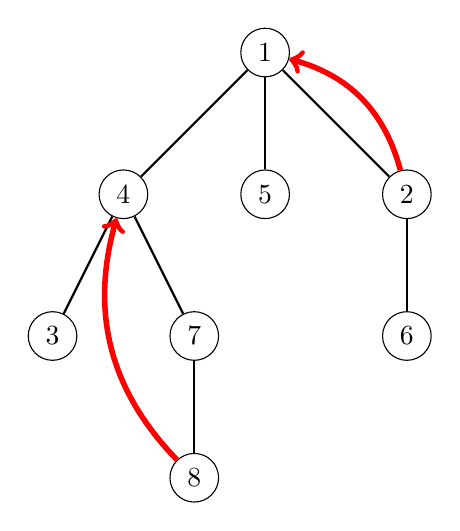
\begin{tikzpicture}[scale=0.9]
\node[draw, circle] (1) at (0,3) {$1$};
\node[draw, circle] (2) at (2,1) {$2$};
\node[draw, circle] (3) at (-2,1) {$4$};
\node[draw, circle] (4) at (0,1) {$5$};
\node[draw, circle] (5) at (2,-1) {$6$};
\node[draw, circle] (6) at (-3,-1) {$3$};
\node[draw, circle] (7) at (-1,-1) {$7$};
\node[draw, circle] (8) at (-1,-3) {$8$};
\path[draw,thick,-] (1) -- (2);
\path[draw,thick,-] (1) -- (3);
\path[draw,thick,-] (1) -- (4);
\path[draw,thick,-] (2) -- (5);
\path[draw,thick,-] (3) -- (6);
\path[draw,thick,-] (3) -- (7);
\path[draw,thick,-] (7) -- (8);

\path[draw=red,thick,->,line width=2pt] (8) edge [bend left] (3);
\path[draw=red,thick,->,line width=2pt] (2) edge [bend right] (1);
\end{tikzpicture}
\end{center}

Una manera fácil de calcular cualquier valor de $\texttt{ancestro}(x,k)$
es realizar una secuencia de $k$ movimientos en el árbol.
Sin embargo, la complejidad temporal de este método
es $O(k)$, que puede ser lenta, porque un árbol de $n$
nodos puede tener una cadena de $n$ nodos.

Afortunadamente, usando una técnica similar a la
usada en el Capítulo 16.3, cualquier valor de $\texttt{ancestro}(x,k)$
puede ser calculado eficientemente en tiempo $O(\log k)$
después del preprocesamiento.
La idea es precalcular todos los valores $\texttt{ancestro}(x,k)$
donde $k \le n$ es una potencia de dos.
Por ejemplo, los valores para el árbol anterior
son los siguientes:

\begin{center}
\begin{tabular}{r|rrrrrrrrr}
$x$ & 1 & 2 & 3 & 4 & 5 & 6 & 7 & 8 \\
\hline
$\texttt{ancestro}(x,1)$ & 0 & 1 & 4 & 1 & 1 & 2 & 4 & 7 \\
$\texttt{ancestro}(x,2)$ & 0 & 0 & 1 & 0 & 0 & 1 & 1 & 4 \\
$\texttt{ancestro}(x,4)$ & 0 & 0 & 0 & 0 & 0 & 0 & 0 & 0 \\
$\cdots$ \\
\end{tabular}
\end{center}

El preprocesamiento toma $O(n \log n)$ tiempo,
porque se calculan $O(\log n)$ valores para cada nodo.
Después de esto, cualquier valor de $\texttt{ancestro}(x,k)$ puede ser calculado
en tiempo $O(\log k)$ representando $k$
como una suma donde cada término es una potencia de dos.

\section{Subárboles y caminos}

\index{arreglo de recorrido de árbol}

Un \key{arreglo de recorrido de árbol} contiene los nodos de un árbol enraizado
en el orden en que una búsqueda en profundidad
desde el nodo raíz los visita.
Por ejemplo, en el árbol
\begin{center}
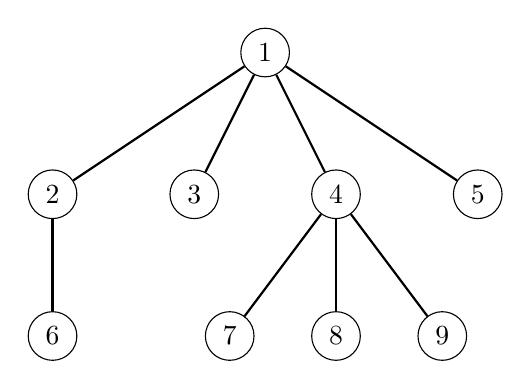
\begin{tikzpicture}[scale=0.9]
\node[draw, circle] (1) at (0,3) {$1$};
\node[draw, circle] (2) at (-3,1) {$2$};
\node[draw, circle] (3) at (-1,1) {$3$};
\node[draw, circle] (4) at (1,1) {$4$};
\node[draw, circle] (5) at (3,1) {$5$};
\node[draw, circle] (6) at (-3,-1) {$6$};
\node[draw, circle] (7) at (-0.5,-1) {$7$};
\node[draw, circle] (8) at (1,-1) {$8$};
\node[draw, circle] (9) at (2.5,-1) {$9$};

\path[draw,thick,-] (1) -- (2);
\path[draw,thick,-] (1) -- (3);
\path[draw,thick,-] (1) -- (4);
\path[draw,thick,-] (1) -- (5);
\path[draw,thick,-] (2) -- (6);
\path[draw,thick,-] (4) -- (7);
\path[draw,thick,-] (4) -- (8);
\path[draw,thick,-] (4) -- (9);
\end{tikzpicture}
\end{center}
una búsqueda en profundidad procede de la siguiente manera:
\begin{center}
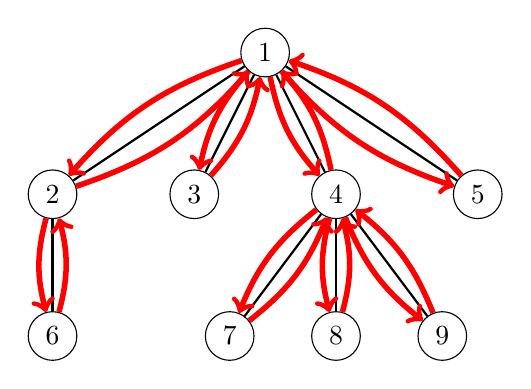
\begin{tikzpicture}[scale=0.9]
\node[draw, circle] (1) at (0,3) {$1$};
\node[draw, circle] (2) at (-3,1) {$2$};
\node[draw, circle] (3) at (-1,1) {$3$};
\node[draw, circle] (4) at (1,1) {$4$};
\node[draw, circle] (5) at (3,1) {$5$};
\node[draw, circle] (6) at (-3,-1) {$6$};
\node[draw, circle] (7) at (-0.5,-1) {$7$};
\node[draw, circle] (8) at (1,-1) {$8$};
\node[draw, circle] (9) at (2.5,-1) {$9$};

\path[draw,thick,-] (1) -- (2);
\path[draw,thick,-] (1) -- (3);
\path[draw,thick,-] (1) -- (4);
\path[draw,thick,-] (1) -- (5);
\path[draw,thick,-] (2) -- (6);
\path[draw,thick,-] (4) -- (7);
\path[draw,thick,-] (4) -- (8);
\path[draw,thick,-] (4) -- (9);



\path[draw=red,thick,->,line width=2pt] (1) edge [bend right=15] (2);
\path[draw=red,thick,->,line width=2pt] (2) edge [bend right=15] (6);
\path[draw=red,thick,->,line width=2pt] (6) edge [bend right=15] (2);
\path[draw=red,thick,->,line width=2pt] (2) edge [bend right=15] (1);
\path[draw=red,thick,->,line width=2pt] (1) edge [bend right=15] (3);
\path[draw=red,thick,->,line width=2pt] (3) edge [bend right=15] (1);
\path[draw=red,thick,->,line width=2pt] (1) edge [bend right=15] (4);
\path[draw=red,thick,->,line width=2pt] (4) edge [bend right=15] (7);
\path[draw=red,thick,->,line width=2pt] (7) edge [bend right=15] (4);
\path[draw=red,thick,->,line width=2pt] (4) edge [bend right=15] (8);
\path[draw=red,thick,->,line width=2pt] (8) edge [bend right=15] (4);
\path[draw=red,thick,->,line width=2pt] (4) edge [bend right=15] (9);
\path[draw=red,thick,->,line width=2pt] (9) edge [bend right=15] (4);
\path[draw=red,thick,->,line width=2pt] (4) edge [bend right=15] (1);
\path[draw=red,thick,->,line width=2pt] (1) edge [bend right=15] (5);
\path[draw=red,thick,->,line width=2pt] (5) edge [bend right=15] (1);

\end{tikzpicture}
\end{center}
Por lo tanto, la matriz de recorrido del árbol correspondiente es la siguiente:
\begin{center}
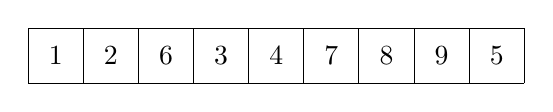
\begin{tikzpicture}[scale=0.7]
\draw (0,0) grid (9,1);

\node at (0.5,0.5) {$1$};
\node at (1.5,0.5) {$2$};
\node at (2.5,0.5) {$6$};
\node at (3.5,0.5) {$3$};
\node at (4.5,0.5) {$4$};
\node at (5.5,0.5) {$7$};
\node at (6.5,0.5) {$8$};
\node at (7.5,0.5) {$9$};
\node at (8.5,0.5) {$5$};
% 
% \footnotesize
% \node at (0.5,1.4) {$1$};
% \node at (1.5,1.4) {$2$};
% \node at (2.5,1.4) {$3$};
% \node at (3.5,1.4) {$4$};
% \node at (4.5,1.4) {$5$};
% \node at (5.5,1.4) {$6$};
% \node at (6.5,1.4) {$7$};
% \node at (7.5,1.4) {$8$};
% \node at (8.5,1.4) {$9$};
\end{tikzpicture}
\end{center}

\subsubsection{Consultas de subárbol}

Cada subárbol de un árbol corresponde a una submatriz
de la matriz de recorrido del árbol de modo que
el primer elemento de la submatriz es el nodo raíz.
Por ejemplo, la siguiente submatriz contiene
los nodos del subárbol del nodo $4$:
\begin{center}
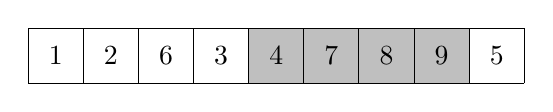
\begin{tikzpicture}[scale=0.7]
\fill[color=lightgray] (4,0) rectangle (8,1);
\draw (0,0) grid (9,1);

\node at (0.5,0.5) {$1$};
\node at (1.5,0.5) {$2$};
\node at (2.5,0.5) {$6$};
\node at (3.5,0.5) {$3$};
\node at (4.5,0.5) {$4$};
\node at (5.5,0.5) {$7$};
\node at (6.5,0.5) {$8$};
\node at (7.5,0.5) {$9$};
\node at (8.5,0.5) {$5$};
% 
% \footnotesize
% \node at (0.5,1.4) {$1$};
% \node at (1.5,1.4) {$2$};
% \node at (2.5,1.4) {$3$};
% \node at (3.5,1.4) {$4$};
% \node at (4.5,1.4) {$5$};
% \node at (5.5,1.4) {$6$};
% \node at (6.5,1.4) {$7$};
% \node at (7.5,1.4) {$8$};
% \node at (8.5,1.4) {$9$};
\end{tikzpicture}
\end{center}
Usando este hecho, podemos procesar eficientemente consultas
que están relacionadas con subárboles de un árbol.
Como ejemplo, considere un problema donde cada nodo
se le asigna un valor, y nuestra tarea es apoyar
las siguientes consultas:
\begin{itemize}
\item actualizar el valor de un nodo
\item calcular la suma de valores en el subárbol de un nodo
\end{itemize}

Considere el siguiente árbol donde los números azules
son los valores de los nodos.
Por ejemplo, la suma del subárbol del nodo $4$
es $3+4+3+1=11$.

\begin{center}
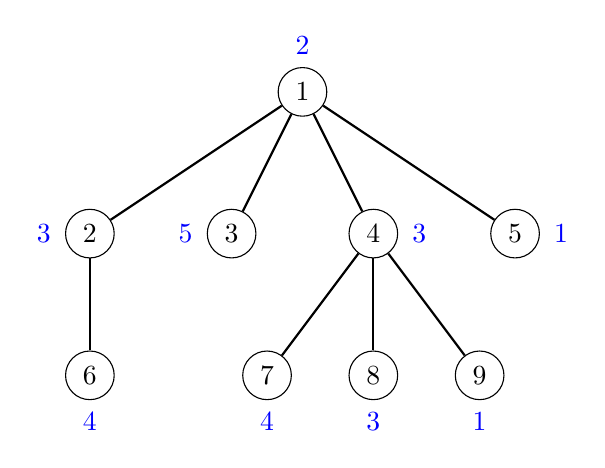
\begin{tikzpicture}[scale=0.9]
\node[draw, circle] (1) at (0,3) {$1$};
\node[draw, circle] (2) at (-3,1) {$2$};
\node[draw, circle] (3) at (-1,1) {$3$};
\node[draw, circle] (4) at (1,1) {$4$};
\node[draw, circle] (5) at (3,1) {$5$};
\node[draw, circle] (6) at (-3,-1) {$6$};
\node[draw, circle] (7) at (-0.5,-1) {$7$};
\node[draw, circle] (8) at (1,-1) {$8$};
\node[draw, circle] (9) at (2.5,-1) {$9$};

\path[draw,thick,-] (1) -- (2);
\path[draw,thick,-] (1) -- (3);
\path[draw,thick,-] (1) -- (4);
\path[draw,thick,-] (1) -- (5);
\path[draw,thick,-] (2) -- (6);
\path[draw,thick,-] (4) -- (7);
\path[draw,thick,-] (4) -- (8);
\path[draw,thick,-] (4) -- (9);

\node[color=blue] at (0,3+0.65) {2};
\node[color=blue] at (-3-0.65,1) {3};
\node[color=blue] at (-1-0.65,1) {5};
\node[color=blue] at (1+0.65,1) {3};
\node[color=blue] at (3+0.65,1) {1};
\node[color=blue] at (-3,-1-0.65) {4};
\node[color=blue] at (-0.5,-1-0.65) {4};
\node[color=blue] at (1,-1-0.65) {3};
\node[color=blue] at (2.5,-1-0.65) {1};
\end{tikzpicture}
\end{center}

La idea es construir una matriz de recorrido del árbol que contiene
tres valores para cada nodo: el identificador del nodo,
el tamaño del subárbol, y el valor del nodo.
Por ejemplo, la matriz para el árbol anterior es la siguiente:

\begin{center}
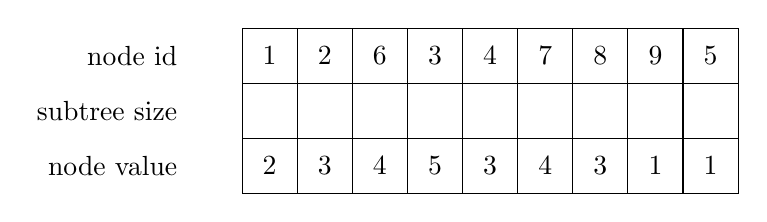
\begin{tikzpicture}[scale=0.7]
\draw (0,1) grid (9,-2);

\node[left] at (-1,0.5) {node id};
\node[left] at (-1,-0.5) {subtree size};
\node[left] at (-1,-1.5) {node value};

\node at (0.5,0.5) {$1$};
\node at (1.5,0.5) {$2$};
\node at (2.5,0.5) {$6$};
\node at (3.5,0.5) {$3$};
\node at (4.5,0.5) {$4$};
\node at (5.5,0.5) {$7$};
\node at (6.5,0.5) {$8$};
\node at (7.5,0.5) {$9$};
\node at (8.5,0.5) {$5$};
\node at (0.5,-1.5) {$2$};
\node at (1.5,-1.5) {$3$};
\node at (2.5,-1.5) {$4$};
\node at (3.5,-1.5) {$5$};
\node at (4.5,-1.5) {$3$};
\node at (5.5,-1.5) {$4$};
\node at (6.5,-1.5) {$3$};
\node at (7.5,-1.5) {$1$};
\node at (8.5,-1.5) {$1$};
% 
% \footnotesize
% \node at (0.5,1.4) {$1$};
% \node at (1.5,1.4) {$2$};
% \node at (2.5,1.4) {$3$};
% \node at (3.5,1.4) {$4$};
% \node at (4.5,1.4) {$5$};
% \node at (5.5,1.4) {$6$};
% \node at (6.5,1.4) {$7$};
% \node at (7.5,1.4) {$8$};
% \node at (8.5,1.4) {$9$};
\end{tikzpicture}
\end{center}

Usando esta matriz, podemos calcular la suma de valores
en cualquier subárbol encontrando primero el tamaño del subárbol
y luego los valores de los nodos correspondientes.
Por ejemplo, los valores en el subárbol del nodo $4$
se pueden encontrar de la siguiente manera:

\begin{center}
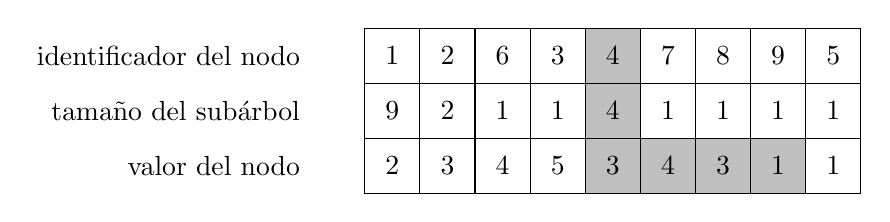
\begin{tikzpicture}[scale=0.7]
\fill[color=lightgray] (4,1) rectangle (5,0);
\fill[color=lightgray] (4,0) rectangle (5,-1);
\fill[color=lightgray] (4,-1) rectangle (8,-2);
\draw (0,1) grid (9,-2);

\node[left] at (-1,0.5) {identificador del nodo};
\node[left] at (-1,-0.5) {tamaño del subárbol};
\node[left] at (-1,-1.5) {valor del nodo};

\node at (0.5,0.5) {$1$};
\node at (1.5,0.5) {$2$};
\node at (2.5,0.5) {$6$};
\node at (3.5,0.5) {$3$};
\node at (4.5,0.5) {$4$};
\node at (5.5,0.5) {$7$};
\node at (6.5,0.5) {$8$};
\node at (7.5,0.5) {$9$};
\node at (8.5,0.5) {$5$};

\node at (0.5,-0.5) {$9$};
\node at (1.5,-0.5) {$2$};
\node at (2.5,-0.5) {$1$};
\node at (3.5,-0.5) {$1$};
\node at (4.5,-0.5) {$4$};
\node at (5.5,-0.5) {$1$};
\node at (6.5,-0.5) {$1$};
\node at (7.5,-0.5) {$1$};
\node at (8.5,-0.5) {$1$};

\node at (0.5,-1.5) {$2$};
\node at (1.5,-1.5) {$3$};
\node at (2.5,-1.5) {$4$};
\node at (3.5,-1.5) {$5$};
\node at (4.5,-1.5) {$3$};
\node at (5.5,-1.5) {$4$};
\node at (6.5,-1.5) {$3$};
\node at (7.5,-1.5) {$1$};
\node at (8.5,-1.5) {$1$};
% 
% \footnotesize
% \node at (0.5,1.4) {$1$};
% \node at (1.5,1.4) {$2$};
% \node at (2.5,1.4) {$3$};
% \node at (3.5,1.4) {$4$};
% \node at (4.5,1.4) {$5$};
% \node at (5.5,1.4) {$6$};
% \node at (6.5,1.4) {$7$};
% \node at (7.5,1.4) {$8$};
% \node at (8.5,1.4) {$9$};
\end{tikzpicture}
\end{center}

Para responder a las consultas de forma eficiente,
basta con almacenar los valores de los
nodos en un árbol binario indexado o un árbol de segmentos.
Después de esto, podemos actualizar un valor
y calcular la suma de los valores en tiempo $O(\log n)$.

\subsubsection{Consultas de ruta}

Usando una matriz de recorrido de árbol, también podemos calcular de manera eficiente
las sumas de valores en
rutas desde el nodo raíz hasta cualquier
nodo del árbol.
Considere un problema donde nuestra tarea
es admitir las siguientes consultas:
\begin{itemize}
\item cambiar el valor de un nodo
\item calcular la suma de valores en una ruta desde
la raíz hasta un nodo
\end{itemize}

Por ejemplo, en el siguiente árbol,
la suma de valores desde el nodo raíz hasta el nodo 7 es
$4+5+5=14$:

\begin{center}
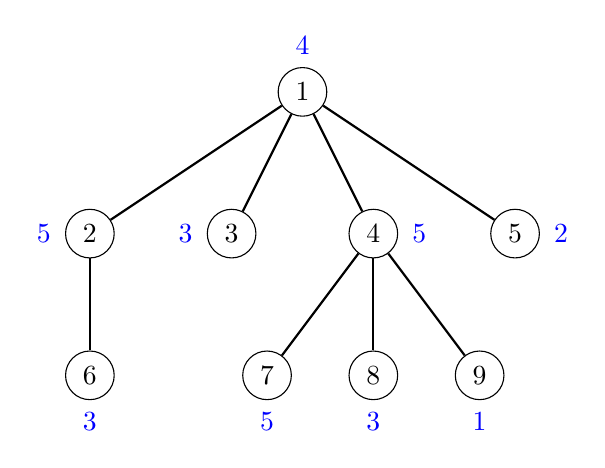
\begin{tikzpicture}[scale=0.9]
\node[draw, circle] (1) at (0,3) {$1$};
\node[draw, circle] (2) at (-3,1) {$2$};
\node[draw, circle] (3) at (-1,1) {$3$};
\node[draw, circle] (4) at (1,1) {$4$};
\node[draw, circle] (5) at (3,1) {$5$};
\node[draw, circle] (6) at (-3,-1) {$6$};
\node[draw, circle] (7) at (-0.5,-1) {$7$};
\node[draw, circle] (8) at (1,-1) {$8$};
\node[draw, circle] (9) at (2.5,-1) {$9$};

\path[draw,thick,-] (1) -- (2);
\path[draw,thick,-] (1) -- (3);
\path[draw,thick,-] (1) -- (4);
\path[draw,thick,-] (1) -- (5);
\path[draw,thick,-] (2) -- (6);
\path[draw,thick,-] (4) -- (7);
\path[draw,thick,-] (4) -- (8);
\path[draw,thick,-] (4) -- (9);

\node[color=blue] at (0,3+0.65) {4};
\node[color=blue] at (-3-0.65,1) {5};
\node[color=blue] at (-1-0.65,1) {3};
\node[color=blue] at (1+0.65,1) {5};
\node[color=blue] at (3+0.65,1) {2};
\node[color=blue] at (-3,-1-0.65) {3};
\node[color=blue] at (-0.5,-1-0.65) {5};
\node[color=blue] at (1,-1-0.65) {3};
\node[color=blue] at (2.5,-1-0.65) {1};
\end{tikzpicture}
\end{center}

Podemos resolver este problema como antes,
pero ahora cada valor en la última fila de la matriz es la suma de valores
en una ruta desde la raíz hasta el nodo.
Por ejemplo, la siguiente matriz corresponde al árbol anterior:
\begin{center}
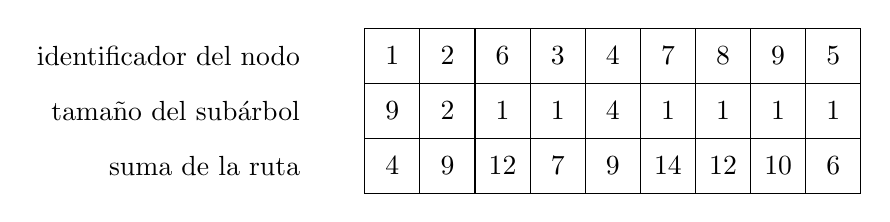
\begin{tikzpicture}[scale=0.7]
\draw (0,1) grid (9,-2);

\node[left] at (-1,0.5) {identificador del nodo};
\node[left] at (-1,-0.5) {tamaño del subárbol};
\node[left] at (-1,-1.5) {suma de la ruta};

\node at (0.5,0.5) {$1$};
\node at (1.5,0.5) {$2$};
\node at (2.5,0.5) {$6$};
\node at (3.5,0.5) {$3$};
\node at (4.5,0.5) {$4$};
\node at (5.5,0.5) {$7$};
\node at (6.5,0.5) {$8$};
\node at (7.5,0.5) {$9$};
\node at (8.5,0.5) {$5$};

\node at (0.5,-0.5) {$9$};
\node at (1.5,-0.5) {$2$};
\node at (2.5,-0.5) {$1$};
\node at (3.5,-0.5) {$1$};
\node at (4.5,-0.5) {$4$};
\node at (5.5,-0.5) {$1$};
\node at (6.5,-0.5) {$1$};
\node at (7.5,-0.5) {$1$};
\node at (8.5,-0.5) {$1$};
\node at (0.5,-1.5) {$4$};
\node at (1.5,-1.5) {$9$};
\node at (2.5,-1.5) {$12$};
\node at (3.5,-1.5) {$7$};
\node at (4.5,-1.5) {$9$};
\node at (5.5,-1.5) {$14$};
\node at (6.5,-1.5) {$12$};
\node at (7.5,-1.5) {$10$};
\node at (8.5,-1.5) {$6$};
\end{tikzpicture}
\end{center}

Cuando el valor de un nodo aumenta en $x$,
las sumas de todos los nodos en su subárbol aumentan en $x$.
Por ejemplo, si el valor del nodo 4 aumenta en 1,
la matriz cambia de la siguiente manera:

\begin{center}
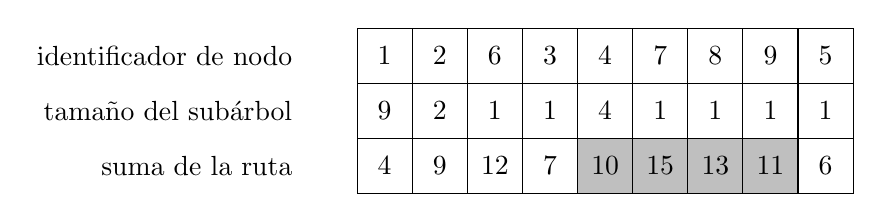
\begin{tikzpicture}[scale=0.7]
\fill[color=lightgray] (4,-1) rectangle (8,-2);
\draw (0,1) grid (9,-2);

\node[left] at (-1,0.5) {identificador de nodo};
\node[left] at (-1,-0.5) {tamaño del subárbol};
\node[left] at (-1,-1.5) {suma de la ruta};

\node at (0.5,0.5) {$1$};
\node at (1.5,0.5) {$2$};
\node at (2.5,0.5) {$6$};
\node at (3.5,0.5) {$3$};
\node at (4.5,0.5) {$4$};
\node at (5.5,0.5) {$7$};
\node at (6.5,0.5) {$8$};
\node at (7.5,0.5) {$9$};
\node at (8.5,0.5) {$5$};

\node at (0.5,-0.5) {$9$};
\node at (1.5,-0.5) {$2$};
\node at (2.5,-0.5) {$1$};
\node at (3.5,-0.5) {$1$};
\node at (4.5,-0.5) {$4$};
\node at (5.5,-0.5) {$1$};
\node at (6.5,-0.5) {$1$};
\node at (7.5,-0.5) {$1$};
\node at (8.5,-0.5) {$1$};

\node at (0.5,-1.5) {$4$};
\node at (1.5,-1.5) {$9$};
\node at (2.5,-1.5) {$12$};
\node at (3.5,-1.5) {$7$};
\node at (4.5,-1.5) {$10$};
\node at (5.5,-1.5) {$15$};
\node at (6.5,-1.5) {$13$};
\node at (7.5,-1.5) {$11$};
\node at (8.5,-1.5) {$6$};
\end{tikzpicture}
\end{center}

Por lo tanto, para soportar ambas operaciones,
deberíamos poder aumentar todos los valores
en un rango y recuperar un solo valor.
Esto se puede hacer en tiempo $O(\log n)$
usando un índice binario
o un árbol de segmentos (ver Capítulo 9.4).

\section{Antepasado común más bajo}

\index{antepasado común más bajo}

El \key{antepasado común más bajo}
de dos nodos de un árbol enraizado es el nodo más bajo
cuyo subárbol contiene ambos nodos.
Un problema típico es procesar de manera eficiente
las consultas que piden encontrar el antepasado común más bajo
de dos nodos.

Por ejemplo, en el siguiente árbol,
el antepasado común más bajo de los nodos 5 y 8
es el nodo 2:
\begin{center}
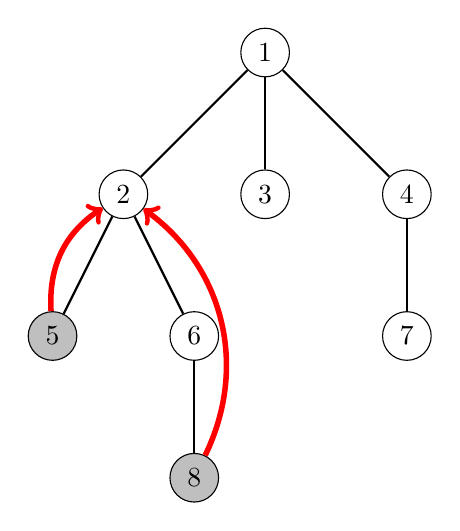
\begin{tikzpicture}[scale=0.9]
\node[draw, circle] (1) at (0,3) {$1$};
\node[draw, circle] (2) at (2,1) {$4$};
\node[draw, circle] (3) at (-2,1) {$2$};
\node[draw, circle] (4) at (0,1) {$3$};
\node[draw, circle] (5) at (2,-1) {$7$};
\node[draw, circle, fill=lightgray] (6) at (-3,-1) {$5$};
\node[draw, circle] (7) at (-1,-1) {$6$};
\node[draw, circle, fill=lightgray] (8) at (-1,-3) {$8$};
\path[draw,thick,-] (1) -- (2);
\path[draw,thick,-] (1) -- (3);
\path[draw,thick,-] (1) -- (4);
\path[draw,thick,-] (2) -- (5);
\path[draw,thick,-] (3) -- (6);
\path[draw,thick,-] (3) -- (7);
\path[draw,thick,-] (7) -- (8);

\path[draw=red,thick,->,line width=2pt] (6) edge [bend left] (3);
\path[draw=red,thick,->,line width=2pt] (8) edge [bend right=40] (3);
\end{tikzpicture}
\end{center}

A continuación, discutiremos dos técnicas eficientes para
encontrar el antepasado común más bajo de dos nodos.

\subsubsection{Método 1}

Una forma de resolver el problema es usar el hecho
de que podemos encontrar eficientemente el $k$-ésimo
antepasado de cualquier nodo en el árbol.
Usando esto, podemos dividir el problema de
encontrar el antepasado común más bajo en dos partes.

Usamos dos punteros que inicialmente apuntan a los
dos nodos cuyo antepasado común más bajo debemos encontrar.
Primero, movemos uno de los punteros hacia arriba
para que ambos punteros apunten a nodos en el mismo nivel.

En el escenario de ejemplo, movemos el segundo puntero un
nivel hacia arriba para que apunte al nodo 6
que está en el mismo nivel que el nodo 5:

\begin{center}
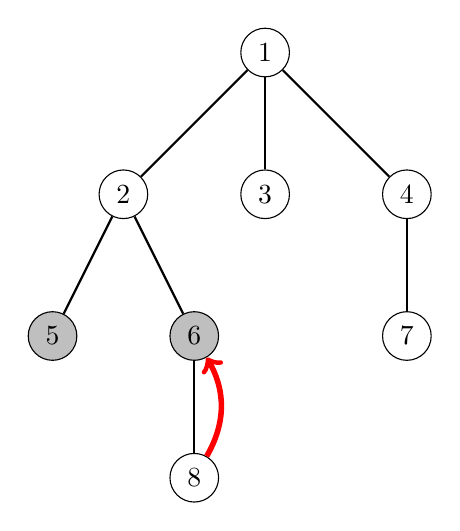
\begin{tikzpicture}[scale=0.9]
\node[draw, circle] (1) at (0,3) {$1$};
\node[draw, circle] (2) at (2,1) {$4$};
\node[draw, circle] (3) at (-2,1) {$2$};
\node[draw, circle] (4) at (0,1) {$3$};
\node[draw, circle] (5) at (2,-1) {$7$};
\node[draw, circle,fill=lightgray] (6) at (-3,-1) {$5$};
\node[draw, circle,fill=lightgray] (7) at (-1,-1) {$6$};
\node[draw, circle] (8) at (-1,-3) {$8$};
\path[draw,thick,-] (1) -- (2);
\path[draw,thick,-] (1) -- (3);
\path[draw,thick,-] (1) -- (4);
\path[draw,thick,-] (2) -- (5);
\path[draw,thick,-] (3) -- (6);
\path[draw,thick,-] (3) -- (7);
\path[draw,thick,-] (7) -- (8);

\path[draw=red,thick,->,line width=2pt] (8) edge [bend right] (7);
\end{tikzpicture}
\end{center}

Después de esto, determinamos el número mínimo de pasos
necesarios para mover ambos punteros hacia arriba para que
apunten al mismo nodo.
El nodo al que apuntan los punteros después de esto
es el antepasado común más bajo.

En el escenario de ejemplo, basta con mover ambos punteros
un paso hacia arriba al nodo 2,
que es el antepasado común más bajo:


\begin{center}
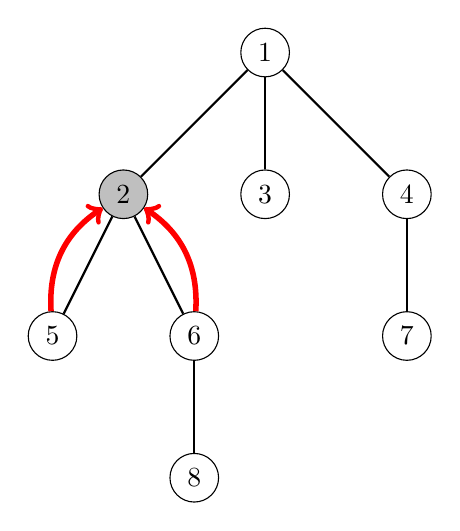
\begin{tikzpicture}[scale=0.9]
\node[draw, circle] (1) at (0,3) {$1$};
\node[draw, circle] (2) at (2,1) {$4$};
\node[draw, circle,fill=lightgray] (3) at (-2,1) {$2$};
\node[draw, circle] (4) at (0,1) {$3$};
\node[draw, circle] (5) at (2,-1) {$7$};
\node[draw, circle] (6) at (-3,-1) {$5$};
\node[draw, circle] (7) at (-1,-1) {$6$};
\node[draw, circle] (8) at (-1,-3) {$8$};
\path[draw,thick,-] (1) -- (2);
\path[draw,thick,-] (1) -- (3);
\path[draw,thick,-] (1) -- (4);
\path[draw,thick,-] (2) -- (5);
\path[draw,thick,-] (3) -- (6);
\path[draw,thick,-] (3) -- (7);
\path[draw,thick,-] (7) -- (8);

\path[draw=red,thick,->,line width=2pt] (6) edge [bend left] (3);
\path[draw=red,thick,->,line width=2pt] (7) edge [bend right] (3);
\end{tikzpicture}
\end{center}

Dado que ambas partes del algoritmo se pueden realizar en
tiempo $O(\log n)$ utilizando información precalculada,
podemos encontrar el ancestro común más bajo de dos
nodos en tiempo $O(\log n)$.

\subsubsection{Método 2}

Otra forma de resolver el problema se basa en
una matriz de recorrido de árbol\footnote{Este algoritmo de ancestro común más bajo se presentó en \cite{ben00}.
Esta técnica a veces se llama la técnica de recorrido de Euler \index{técnica de recorrido de Euler}
\key{técnica de recorrido de Euler} \cite{tar84}.}.
Una vez más, la idea es recorrer los nodos
utilizando una búsqueda en profundidad:

\begin{center}
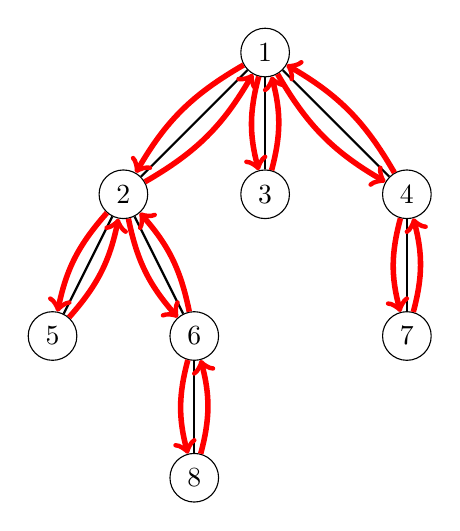
\begin{tikzpicture}[scale=0.9]
\node[draw, circle] (1) at (0,3) {$1$};
\node[draw, circle] (2) at (2,1) {$4$};
\node[draw, circle] (3) at (-2,1) {$2$};
\node[draw, circle] (4) at (0,1) {$3$};
\node[draw, circle] (5) at (2,-1) {$7$};
\node[draw, circle] (6) at (-3,-1) {$5$};
\node[draw, circle] (7) at (-1,-1) {$6$};
\node[draw, circle] (8) at (-1,-3) {$8$};
\path[draw,thick,-] (1) -- (2);
\path[draw,thick,-] (1) -- (3);
\path[draw,thick,-] (1) -- (4);
\path[draw,thick,-] (2) -- (5);
\path[draw,thick,-] (3) -- (6);
\path[draw,thick,-] (3) -- (7);
\path[draw,thick,-] (7) -- (8);

\path[draw=red,thick,->,line width=2pt] (1) edge [bend right=15] (3);
\path[draw=red,thick,->,line width=2pt] (3) edge [bend right=15] (6);
\path[draw=red,thick,->,line width=2pt] (6) edge [bend right=15] (3);
\path[draw=red,thick,->,line width=2pt] (3) edge [bend right=15] (7);
\path[draw=red,thick,->,line width=2pt] (7) edge [bend right=15] (8);
\path[draw=red,thick,->,line width=2pt] (8) edge [bend right=15] (7);
\path[draw=red,thick,->,line width=2pt] (7) edge [bend right=15] (3);
\path[draw=red,thick,->,line width=2pt] (3) edge [bend right=15] (1);
\path[draw=red,thick,->,line width=2pt] (1) edge [bend right=15] (4);
\path[draw=red,thick,->,line width=2pt] (4) edge [bend right=15] (1);
\path[draw=red,thick,->,line width=2pt] (1) edge [bend right=15] (2);
\path[draw=red,thick,->,line width=2pt] (2) edge [bend right=15] (5);
\path[draw=red,thick,->,line width=2pt] (5) edge [bend right=15] (2);
\path[draw=red,thick,->,line width=2pt] (2) edge [bend right=15] (1);
\end{tikzpicture}
\end{center}

Sin embargo, usamos una matriz de recorrido de árbol diferente a la anterior:
agregamos cada nodo a la matriz \emph{siempre}
cuando la búsqueda en profundidad recorre el nodo,
y no solo en la primera visita.
Por lo tanto, un nodo que tiene $k$ hijos aparece $k+1$ veces
en la matriz y hay un total de $2n-1$
nodos en la matriz.

Almacenamos dos valores en la matriz:
el identificador del nodo y la profundidad del 
nodo en el árbol.
La siguiente matriz corresponde al árbol anterior:

\begin{center}
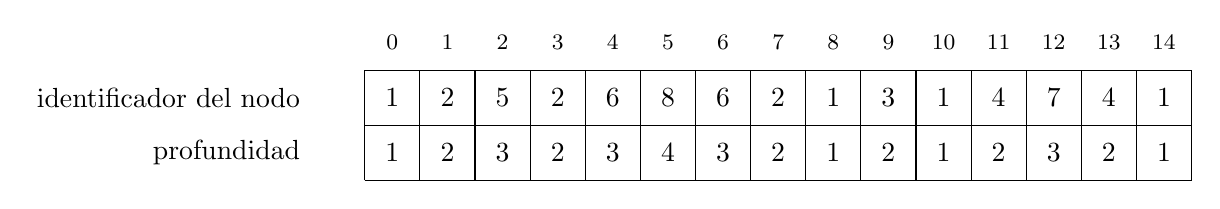
\begin{tikzpicture}[scale=0.7]

\node[left] at (-1,1.5) {identificador del nodo};
\node[left] at (-1,0.5) {profundidad};

\draw (0,1) grid (15,2);
\node at (0.5,1.5) {$1$};
\node at (1.5,1.5) {$2$};
\node at (2.5,1.5) {$5$};
\node at (3.5,1.5) {$2$};
\node at (4.5,1.5) {$6$};
\node at (5.5,1.5) {$8$};
\node at (6.5,1.5) {$6$};
\node at (7.5,1.5) {$2$};
\node at (8.5,1.5) {$1$};
\node at (9.5,1.5) {$3$};
\node at (10.5,1.5) {$1$};
\node at (11.5,1.5) {$4$};
\node at (12.5,1.5) {$7$};
\node at (13.5,1.5) {$4$};
\node at (14.5,1.5) {$1$};

\draw (0,0) grid (15,1);
\node at (0.5,0.5) {$1$};
\node at (1.5,0.5) {$2$};
\node at (2.5,0.5) {$3$};
\node at (3.5,0.5) {$2$};
\node at (4.5,0.5) {$3$};
\node at (5.5,0.5) {$4$};
\node at (6.5,0.5) {$3$};
\node at (7.5,0.5) {$2$};
\node at (8.5,0.5) {$1$};
\node at (9.5,0.5) {$2$};
\node at (10.5,0.5) {$1$};
\node at (11.5,0.5) {$2$};
\node at (12.5,0.5) {$3$};
\node at (13.5,0.5) {$2$};
\node at (14.5,0.5) {$1$};

\footnotesize
\node at (0.5,2.5) {$0$};
\node at (1.5,2.5) {$1$};
\node at (2.5,2.5) {$2$};
\node at (3.5,2.5) {$3$};
\node at (4.5,2.5) {$4$};
\node at (5.5,2.5) {$5$};
\node at (6.5,2.5) {$6$};
\node at (7.5,2.5) {$7$};
\node at (8.5,2.5) {$8$};
\node at (9.5,2.5) {$9$};
\node at (10.5,2.5) {$10$};
\node at (11.5,2.5) {$11$};
\node at (12.5,2.5) {$12$};
\node at (13.5,2.5) {$13$};
\node at (14.5,2.5) {$14$};
\end{tikzpicture}
\end{center}


Ahora podemos encontrar el antepasado común más bajo
de los nodos $a$ y $b$ encontrando el nodo con la profundidad \emph{mínima}
entre los nodos $a$ y $b$ en el array.
Por ejemplo, el antepasado común más bajo de los nodos $5$ y $8$
se puede encontrar de la siguiente manera:

\begin{center}
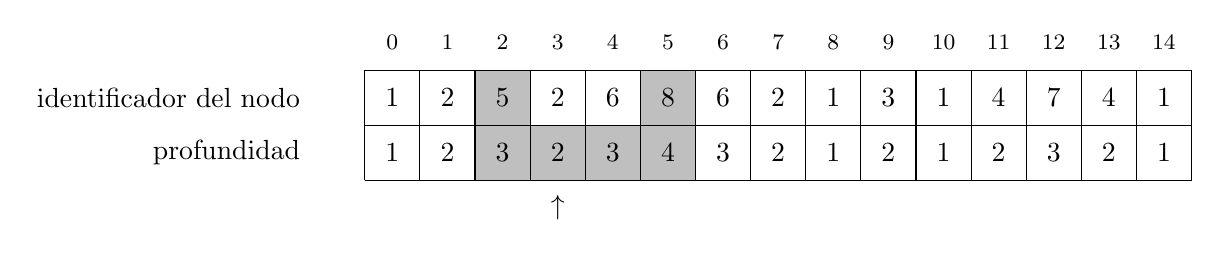
\begin{tikzpicture}[scale=0.7]

\node[left] at (-1,1.5) {identificador del nodo};
\node[left] at (-1,0.5) {profundidad};

\fill[color=lightgray] (2,1) rectangle (3,2);
\fill[color=lightgray] (5,1) rectangle (6,2);
\fill[color=lightgray] (2,0) rectangle (6,1);

\node at (3.5,-0.5) {$\uparrow$};

\draw (0,1) grid (15,2);
\node at (0.5,1.5) {$1$};
\node at (1.5,1.5) {$2$};
\node at (2.5,1.5) {$5$};
\node at (3.5,1.5) {$2$};
\node at (4.5,1.5) {$6$};
\node at (5.5,1.5) {$8$};
\node at (6.5,1.5) {$6$};
\node at (7.5,1.5) {$2$};
\node at (8.5,1.5) {$1$};
\node at (9.5,1.5) {$3$};
\node at (10.5,1.5) {$1$};
\node at (11.5,1.5) {$4$};
\node at (12.5,1.5) {$7$};
\node at (13.5,1.5) {$4$};
\node at (14.5,1.5) {$1$};


\draw (0,0) grid (15,1);
\node at (0.5,0.5) {$1$};
\node at (1.5,0.5) {$2$};
\node at (2.5,0.5) {$3$};
\node at (3.5,0.5) {$2$};
\node at (4.5,0.5) {$3$};
\node at (5.5,0.5) {$4$};
\node at (6.5,0.5) {$3$};
\node at (7.5,0.5) {$2$};
\node at (8.5,0.5) {$1$};
\node at (9.5,0.5) {$2$};
\node at (10.5,0.5) {$1$};
\node at (11.5,0.5) {$2$};
\node at (12.5,0.5) {$3$};
\node at (13.5,0.5) {$2$};
\node at (14.5,0.5) {$1$};

\footnotesize
\node at (0.5,2.5) {$0$};
\node at (1.5,2.5) {$1$};
\node at (2.5,2.5) {$2$};
\node at (3.5,2.5) {$3$};
\node at (4.5,2.5) {$4$};
\node at (5.5,2.5) {$5$};
\node at (6.5,2.5) {$6$};
\node at (7.5,2.5) {$7$};
\node at (8.5,2.5) {$8$};
\node at (9.5,2.5) {$9$};
\node at (10.5,2.5) {$10$};
\node at (11.5,2.5) {$11$};
\node at (12.5,2.5) {$12$};
\node at (13.5,2.5) {$13$};
\node at (14.5,2.5) {$14$};
\end{tikzpicture}
\end{center}

El nodo 5 está en la posición 2, el nodo 8 está en la posición 5,
y el nodo con la profundidad mínima entre
las posiciones $2 \ldots 5$ es el nodo 2 en la posición 3
cuya profundidad es 2.
Por lo tanto, el antepasado común más bajo de
los nodos 5 y 8 es el nodo 2.

Por lo tanto, para encontrar el antepasado común más bajo
de dos nodos, basta con procesar una consulta de rango mínimo.
Como el array es estático,
podemos procesar tales consultas en tiempo $O(1)$
después de un preprocesamiento de tiempo $O(n \log n)$.

\subsubsection{Distancias de los nodos}

La distancia entre los nodos $a$ y $b$
es igual a la longitud del camino de $a$ a $b$.
Resulta que el problema de calcular
la distancia entre los nodos se reduce a
encontrar su antepasado común más bajo.

Primero, enraízamos el árbol arbitrariamente.
Después de esto, la distancia de los nodos $a$ y $b$
se puede calcular usando la fórmula
\[\texttt{profundidad}(a)+\texttt{profundidad}(b)-2 \cdot \texttt{profundidad}(c),\]
donde $c$ es el antepasado común más bajo de $a$ y $b$
y $\texttt{profundidad}(s)$ denota la profundidad del nodo $s$.
Por ejemplo, considere la distancia de los nodos 5 y 8:
\begin{center}
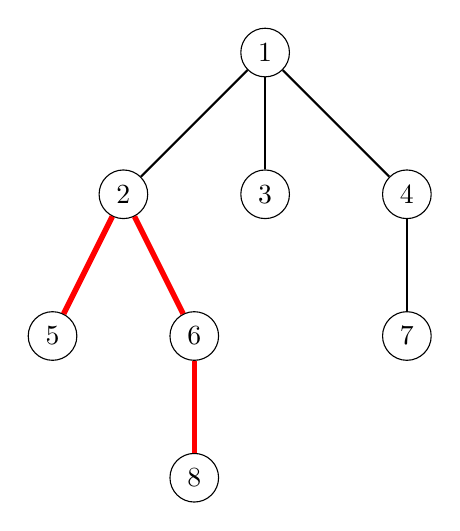
\begin{tikzpicture}[scale=0.9]
\node[draw, circle] (1) at (0,3) {$1$};
\node[draw, circle] (2) at (2,1) {$4$};
\node[draw, circle] (3) at (-2,1) {$2$};
\node[draw, circle] (4) at (0,1) {$3$};
\node[draw, circle] (5) at (2,-1) {$7$};
\node[draw, circle] (6) at (-3,-1) {$5$};
\node[draw, circle] (7) at (-1,-1) {$6$};
\node[draw, circle] (8) at (-1,-3) {$8$};
\path[draw,thick,-] (1) -- (2);
\path[draw,thick,-] (1) -- (3);
\path[draw,thick,-] (1) -- (4);
\path[draw,thick,-] (2) -- (5);
\path[draw,thick,-] (3) -- (6);
\path[draw,thick,-] (3) -- (7);
\path[draw,thick,-] (7) -- (8);

\path[draw=red,thick,-,line width=2pt] (8) -- node[font=\small] {} (7);
\path[draw=red,thick,-,line width=2pt] (7) -- node[font=\small] {} (3);
\path[draw=red,thick,-,line width=2pt] (6) -- node[font=\small] {} (3);
\end{tikzpicture}
\end{center}

El antepasado común más bajo de los nodos 5 y 8 es el nodo 2.
Las profundidades de los nodos son
$\texttt{profundidad}(5)=3$, $\texttt{profundidad}(8)=4$ y $\texttt{profundidad}(2)=2$,
por lo que la distancia entre los nodos 5 y 8 es
$3+4-2\cdot2=3$.

\section{Algoritmos fuera de línea}

Hasta ahora, hemos discutido algoritmos \emph{en línea}
para consultas de árboles.
Esos algoritmos son capaces de procesar
consultas una tras otra de modo que
cada consulta se responda antes de recibir la siguiente consulta.

Sin embargo, en muchos problemas, la propiedad en línea
no es necesaria.
En esta sección, nos centramos en algoritmos \emph{fuera de línea}.
Esos algoritmos reciben un conjunto de consultas que pueden
ser respondidas en cualquier orden.
A menudo es más fácil diseñar un algoritmo fuera de línea
en comparación con un algoritmo en línea.

\subsubsection{Fusión de estructuras de datos}

Un método para construir un algoritmo fuera de línea
es realizar un recorrido en profundidad del árbol
y mantener estructuras de datos en los nodos.
En cada nodo $s$, creamos una estructura de datos
$\texttt{d}[s]$ que se basa en las
estructuras de datos de los hijos de $s$.
Entonces, usando esta estructura de datos,
se procesan todas las consultas relacionadas con $s$.


Como ejemplo, considere el siguiente problema:
Se nos da un árbol donde cada nodo tiene algún valor.
Nuestra tarea es procesar consultas de la forma
''calcular el número de nodos con valor $x$
en el subárbol del nodo $s$''.
Por ejemplo, en el siguiente árbol,
el subárbol del nodo $4$ contiene dos nodos
cuyo valor es 3.

\begin{center}
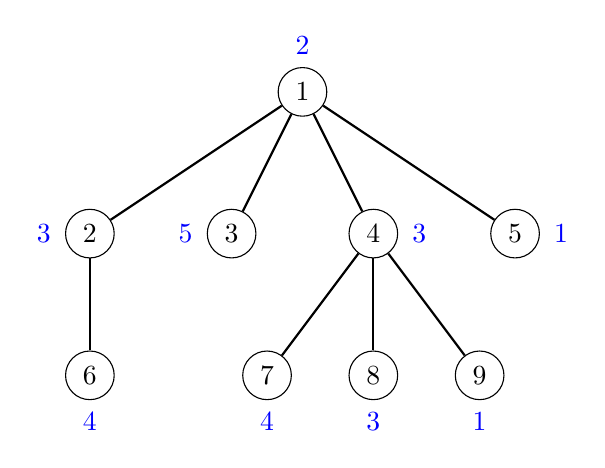
\begin{tikzpicture}[scale=0.9]
\node[draw, circle] (1) at (0,3) {$1$};
\node[draw, circle] (2) at (-3,1) {$2$};
\node[draw, circle] (3) at (-1,1) {$3$};
\node[draw, circle] (4) at (1,1) {$4$};
\node[draw, circle] (5) at (3,1) {$5$};
\node[draw, circle] (6) at (-3,-1) {$6$};
\node[draw, circle] (7) at (-0.5,-1) {$7$};
\node[draw, circle] (8) at (1,-1) {$8$};
\node[draw, circle] (9) at (2.5,-1) {$9$};

\path[draw,thick,-] (1) -- (2);
\path[draw,thick,-] (1) -- (3);
\path[draw,thick,-] (1) -- (4);
\path[draw,thick,-] (1) -- (5);
\path[draw,thick,-] (2) -- (6);
\path[draw,thick,-] (4) -- (7);
\path[draw,thick,-] (4) -- (8);
\path[draw,thick,-] (4) -- (9);

\node[color=blue] at (0,3+0.65) {2};
\node[color=blue] at (-3-0.65,1) {3};
\node[color=blue] at (-1-0.65,1) {5};
\node[color=blue] at (1+0.65,1) {3};
\node[color=blue] at (3+0.65,1) {1};
\node[color=blue] at (-3,-1-0.65) {4};
\node[color=blue] at (-0.5,-1-0.65) {4};
\node[color=blue] at (1,-1-0.65) {3};
\node[color=blue] at (2.5,-1-0.65) {1};
\end{tikzpicture}
\end{center}

En este problema, podemos usar estructuras de mapa
para responder a las consultas.
Por ejemplo, los mapas para el nodo 4 y
sus hijos son los siguientes:

\begin{center}
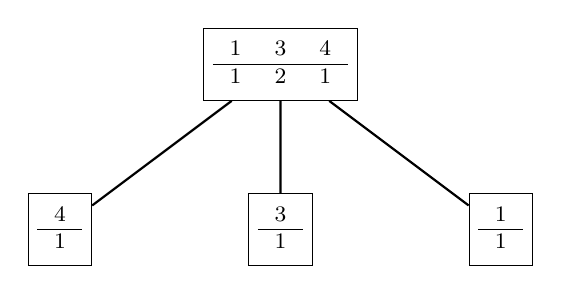
\begin{tikzpicture}[scale=0.7]

\node[draw, rectangle] (a) at (4,5.5)
{
\footnotesize
\begin{tabular}{rrr}
4 \\
\hline
1 \\
\end{tabular}};

\node[draw, rectangle] (b) at (8,5.5)
{
\footnotesize
\begin{tabular}{rrr}
3 \\
\hline
1 \\
\end{tabular}};


\node[draw, rectangle] (c) at (12,5.5)
{
\footnotesize
\begin{tabular}{rr}
1 \\
\hline
1 \\
\end{tabular}};

\node[draw, rectangle] (d) at (8,8.5)
{
\footnotesize
\begin{tabular}{rrr}
1 & 3 & 4 \\
\hline
1 & 2 & 1 \\
\end{tabular}};
\path[draw,thick,-] (a) -- (d);
\path[draw,thick,-] (b) -- (d);
\path[draw,thick,-] (c) -- (d);
\end{tikzpicture}
\end{center}

Si creamos tal estructura de datos para cada nodo,
podemos procesar fácilmente todas las consultas dadas,
porque podemos manejar todas las consultas relacionadas
con un nodo inmediatamente después de crear su
estructura de datos. Por ejemplo, lo anterior
estructura de mapa para el nodo 4
nos dice que su subárbol
contiene dos nodos cuyo valor es 3.

Sin embargo, sería demasiado lento crear
todas las estructuras de datos desde cero.
En cambio, en cada nodo $s$,
creamos una estructura de datos inicial $\texttt{d}[s]$
que solo contiene el valor de $s$.
Después de esto, revisamos los hijos de $s$ y
\emph{fusionamos} $\texttt{d}[s]$ y
todas las estructuras de datos
$\texttt{d}[u]$ donde $u$ es un hijo de $s$.

Por ejemplo, en el árbol anterior, el mapa
para el nodo $4$ se crea fusionando los siguientes mapas:

\begin{center}
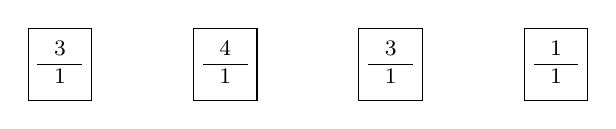
\begin{tikzpicture}[scale=0.7]

\node[draw, rectangle] (a) at (4,5.5)
{
\footnotesize
\begin{tabular}{rrr}
4 \\
\hline
1 \\
\end{tabular}};

\node[draw, rectangle] (b) at (7,5.5)
{
\footnotesize
\begin{tabular}{rrr}
3 \\
\hline
1 \\
\end{tabular}};

\node[draw, rectangle] (c) at (10,5.5)
{
\footnotesize
\begin{tabular}{rr}
1 \\
\hline
1 \\
\end{tabular}};

\node[draw, rectangle] (d) at (1,5.5)
{
\footnotesize
\begin{tabular}{rr}
3 \\
\hline
1 \\
\end{tabular}};

\end{tikzpicture}
\end{center}

Aquí, el primer mapa es la estructura de datos inicial
para el nodo 4,
y los otros tres mapas corresponden a los nodos 7, 8 y 9.

La fusión en el nodo $s$ se puede hacer de la siguiente manera:
Recorremos los hijos de $s$
y en cada hijo $u$ fusionamos $\texttt{d}[s]$
y $\texttt{d}[u]$.
Siempre copiamos el contenido de $\texttt{d}[u]$
a $\texttt{d}[s]$.
Sin embargo, antes de esto, \emph{intercambiamos}
el contenido de $\texttt{d}[s]$ y $\texttt{d}[u]$
si $\texttt{d}[s]$ es menor que $\texttt{d}[u]$.
Al hacer esto, cada valor se copia solo $O(\log n)$
veces durante el recorrido del árbol,
lo que garantiza que el algoritmo sea eficiente.

Para intercambiar el contenido de dos estructuras de datos $a$ y $b$
de manera eficiente, solo podemos usar el siguiente código:
\begin{lstlisting}
swap(a,b);
\end{lstlisting}
Está garantizado que el código anterior funciona en tiempo constante
cuando $a$ y $b$ son estructuras de datos de la biblioteca estándar de C++.

\subsubsection{Antepasados comunes más bajos}

También existe un algoritmo fuera de línea
para procesar un conjunto de
consultas de antepasados comunes más bajos\footnote{Este
algoritmo fue publicado por R. E. Tarjan en 1979 \cite{tar79}.}.
El algoritmo se basa en la estructura de datos union-find
(ver Capítulo 15.2), y el beneficio del algoritmo es
que es más fácil de implementar que
los algoritmos discutidos anteriormente en este capítulo.
El algoritmo se le da como entrada un conjunto de pares de nodos,
y determina para cada uno de estos pares el
antepasado común más bajo de los nodos.
El algoritmo realiza un recorrido en profundidad del árbol
y mantiene conjuntos disjuntos de nodos.
Inicialmente, cada nodo pertenece a un conjunto separado.
Para cada conjunto, también almacenamos el nodo más alto en el
árbol que pertenece al conjunto.

Cuando el algoritmo visita un nodo $x$,
recorre todos los nodos $y$ tales que
el antepasado común más bajo de $x$ e $y$
tiene que ser encontrado.
Si $y$ ya ha sido visitado,
el algoritmo informa que el
antepasado común más bajo de $x$ e $y$
es el nodo más alto en el conjunto de $y$.
Luego, después de procesar el nodo $x$,
el algoritmo une los conjuntos de $x$ y su padre.

Por ejemplo, suponga que queremos encontrar el más bajo
antepasados comunes de pares de nodos $(5,8)$
y $(2,7)$ en el siguiente árbol:
\begin{center}
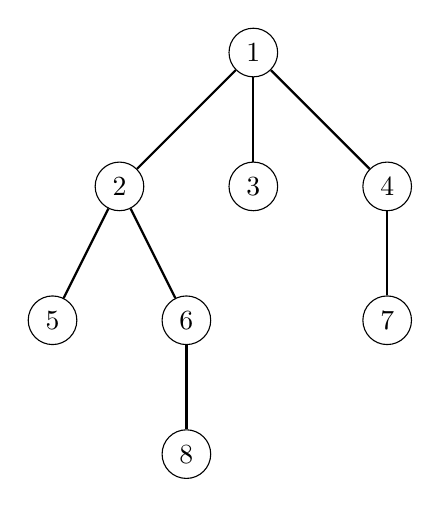
\begin{tikzpicture}[scale=0.85]
\node[draw, circle] (1) at (0,3) {$1$};
\node[draw, circle] (2) at (2,1) {$4$};
\node[draw, circle] (3) at (-2,1) {$2$};
\node[draw, circle] (4) at (0,1) {$3$};
\node[draw, circle] (5) at (2,-1) {$7$};
\node[draw, circle] (6) at (-3,-1) {$5$};
\node[draw, circle] (7) at (-1,-1) {$6$};
\node[draw, circle] (8) at (-1,-3) {$8$};
\path[draw,thick,-] (1) -- (2);
\path[draw,thick,-] (1) -- (3);
\path[draw,thick,-] (1) -- (4);
\path[draw,thick,-] (2) -- (5);
\path[draw,thick,-] (3) -- (6);
\path[draw,thick,-] (3) -- (7);
\path[draw,thick,-] (7) -- (8);
\end{tikzpicture}
\end{center}

En los siguientes árboles, los nodos grises denotan nodos visitados
y los grupos de nodos discontinuos pertenecen al mismo conjunto.
Cuando el algoritmo visita el nodo 8, observa que
el nodo 5 ha sido visitado y el nodo más alto
en su conjunto es 2. Por lo tanto, el antepasado común más bajo
de los nodos 5 y 8 es 2:
\begin{center}
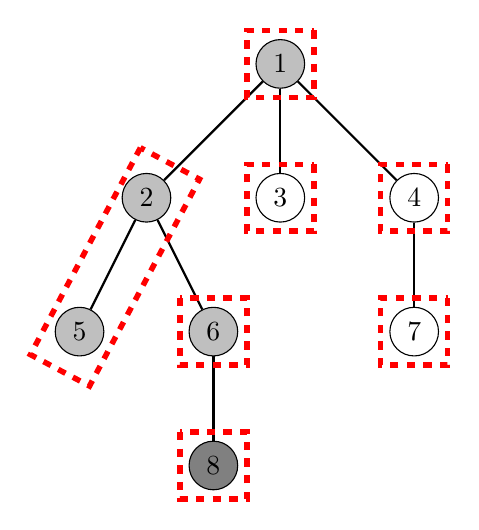
\begin{tikzpicture}[scale=0.85]
\node[draw, circle, fill=lightgray] (1) at (0,3) {$1$};
\node[draw, circle] (2) at (2,1) {$4$};
\node[draw, circle, fill=lightgray] (3) at (-2,1) {$2$};
\node[draw, circle] (4) at (0,1) {$3$};
\node[draw, circle] (5) at (2,-1) {$7$};
\node[draw, circle, fill=lightgray] (6) at (-3,-1) {$5$};
\node[draw, circle, fill=lightgray] (7) at (-1,-1) {$6$};
\node[draw, circle, fill=gray] (8) at (-1,-3) {$8$};
\path[draw,thick,-] (1) -- (2);
\path[draw,thick,-] (1) -- (3);
\path[draw,thick,-] (1) -- (4);
\path[draw,thick,-] (2) -- (5);
\path[draw,thick,-] (3) -- (6);
\path[draw,thick,-] (3) -- (7);
\path[draw,thick,-] (7) -- (8);

\draw [red,thick,dashed,line width=2pt,rotate around={-28:(-2,0)}] (-2.9,1.5) rectangle (-1.9,-2);


\draw [red,thick,dashed,line width=2pt] (-1.5,-0.5) rectangle (-0.5,-1.5);
\draw [red,thick,dashed,line width=2pt] (-1.5,-2.5) rectangle (-0.5,-3.5);

\draw [red,thick,dashed,line width=2pt] (0.5,3.5) rectangle (-0.5,2.5);
\draw [red,thick,dashed,line width=2pt] (0.5,1.5) rectangle (-0.5,0.5);
\draw [red,thick,dashed,line width=2pt] (2.5,1.5) rectangle (1.5,0.5);
\draw [red,thick,dashed,line width=2pt] (2.5,-0.5) rectangle (1.5,-1.5);
\end{tikzpicture}
\end{center}

Más tarde, al visitar el nodo 7,
el algoritmo determina que
el antepasado común más bajo de los nodos 2 y 7 es 1:
\begin{center}
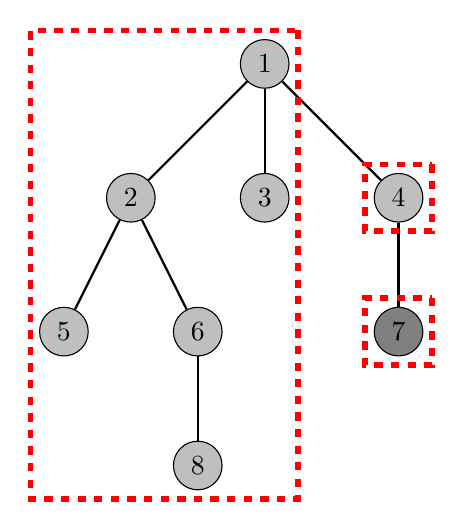
\begin{tikzpicture}[scale=0.85]
\node[draw, circle, fill=lightgray] (1) at (0,3) {$1$};
\node[draw, circle, fill=lightgray] (2) at (2,1) {$4$};
\node[draw, circle, fill=lightgray] (3) at (-2,1) {$2$};
\node[draw, circle, fill=lightgray] (4) at (0,1) {$3$};
\node[draw, circle, fill=gray] (5) at (2,-1) {$7$};
\node[draw, circle, fill=lightgray] (6) at (-3,-1) {$5$};
\node[draw, circle, fill=lightgray] (7) at (-1,-1) {$6$};
\node[draw, circle, fill=lightgray] (8) at (-1,-3) {$8$};
\path[draw,thick,-] (1) -- (2);
\path[draw,thick,-] (1) -- (3);
\path[draw,thick,-] (1) -- (4);
\path[draw,thick,-] (2) -- (5);
\path[draw,thick,-] (3) -- (6);
\path[draw,thick,-] (3) -- (7);
\path[draw,thick,-] (7) -- (8);

\draw [red,thick,dashed,line width=2pt] (0.5,3.5) rectangle (-3.5,-3.5);
\draw [red,thick,dashed,line width=2pt] (2.5,1.5) rectangle (1.5,0.5);
\draw [red,thick,dashed,line width=2pt] (2.5,-0.5) rectangle (1.5,-1.5);

\end{tikzpicture}
\end{center}
